\section{Mô hình đĩa Poincare. Ánh xạ bảo giác}
\subsection{Mô hình đĩa Poincare}
\begin{defn}[Đĩa đơn vị]
    Tập $\U = \{z\in \C ~|~|z| < 1\}$ được gọi là đĩa đơn vị trong mặt phẳng phức $\C$.
\end{defn}
    Ta sẽ xây dựng các đối tượng của hình học hyperbolic trên đĩa đơn vị này và chuyển tất cả các thông tin hình học hyperbolic trong $\hh$ lên đĩa đơn vị $\U$.

\begin{lem}\label{lem 2.3.2}
    Ánh xạ $f(z) = \dfrac{iz+1}{z+i}$ là một vi phôi từ $\hh$ lên đĩa đơn vị $\U$.
\end{lem}
\begin{proof}
    Ta có $f$ là một ánh xạ phân tuyến tính khả vi với $f'(z) = \dfrac{-2}{(z+i)^2} \neq 0$ nên nó là một song ánh liên tục. Hơn nữa $f^{-1}(z) = \dfrac{iz-1}{-z+i}$ cũng là một ánh xạ khả vi trên $\overline{\C}$. 
    
    Chứng tỏ $f$ là một vi phôi trên $\C$.
     \begin{enumerate}
         \item Với mọi $z \in \hh$, tức $\im(z) >0$ thì $f(z) \in \U$.
         Thật vậy,
         \begin{align*}
            |f(z)| &=\sqrt{\left(\dfrac{iz+1}{z+i}\right)\overline{\left(\dfrac{iz+1}{z+i}\right)}}
             % = \dfrac{(iz+1)(-i\overline{z}+1)}{(z+i)(\overline{z}-i)}
             % = \dfrac{z\overline{z}+iz-i\overline{z}+1}{z\overline{z}-iz+i\overline{z}+1}
             = \sqrt{\dfrac{|z|^2-2\im(z) +1}{|z|^2+2\im(z) +1}} < 1\cdot
        \end{align*}
        % Mà $\im(z) > 0$  nên 
        % \[|z|^2+2\im(z) +1 >  (\im(z) - 1)^2 + (\re(z))^2 \geq 0, \] 
        % chứng tỏ $|f(z)|^2 < 1$, tức là $|f(z)| < 1$.
        \item Với mọi $z \in \U$, tức $|z| < 1$ thì $w=f^{-1}(z) \in \hh$. Thật vậy,
        \begin{align*}
            \im(w) = \dfrac{w - \overline{w}}{2i} 
            = \dfrac{1}{2i}\left(\dfrac{iz-1}{-z+i} - \dfrac{-i\overline{z}-1}{-\overline{z}-i}\right)
            = \dfrac{1}{|-z+i|^2} > 0.
        \end{align*}
     \end{enumerate}
    Vì vậy $f$ là một vi phôi từ $\hh$ lên đĩa đơn vị $\U$.
\end{proof}
\begin{remark*}
    Ta sẽ sử dụng vi phôi $f(z) = \dfrac{iz+1}{z+i}$ nói trên để chuyển tất cả các thông tin hình học hyperbolic của $\hh$ như metric, trắc địa, đẳng cự lên đĩa đơn vị $\U$.
\end{remark*}
\begin{defn}[Metric trên $\U$]
    Với mọi $z,w \in \U$ thì $f^{-1}(z),~f^{-1}(w) \in \hh$. Khi đó \[\rho^*(z,w) \defeq \rho(f^{-1}(z), f^{-1}(w))\]
    là một metric trên $\U$.
\end{defn}
\begin{proof}
    Ta sẽ chứng minh $\rho^*$ được định nghĩa như trên là một metric trên $\U$ bằng cách chỉ ra nó thoả mãn 3 tiên đề của một metric như sau
    \begin{enumerate}
        \item (Tính xác định dương) Với mọi $z,w \in \U$ thì $\rho^*(z,w) = \rho(f^{-1}(z), f^{-1}(w))\geq 0$, hơn nữa 
        \[\rho^*(z,w) = 0 \Leftrightarrow \rho(f^{-1}(z), f^{-1}(w)) = 0 \Leftrightarrow f^{-1}(z) = f^{-1}(w) \Leftrightarrow z = w.\]
        \item (Tính đối xứng) Do $\rho$ là một metric trên $\hh$ nên nó đối xứng, do đó vơi mọi $z, w \in \U$ thì 
        \[\rho^*(w,z) = \rho(f^{-1}(w), f^{-1}(z)) = \rho(f^{-1}(z), f^{-1}(w)) = \rho^*(z,w)\]
        \item (Bất đẳng thức tam giác) Với mọi $z,w,u \in \U$ thì 
        \[\rho(f^{-1}(z), f^{-1}(w)) + \rho(f^{-1}(w), f^{-1}(u)) \geq \rho(f^{-1}(z), f^{-1}(u)).\]
        Tức $\rho^*(z,w) + \rho^*(w,u) \geq \rho^*(z,u).$
    \end{enumerate}
\end{proof}
% \begin{defn}(Độ dài hyperbolic trong $\U$)
% \end{defn}
% \begin{lem}
%     Với $z \in \hh$ và $f(z) = \dfrac{zi+1}{z+i}$ thì $\dfrac{2|f'(z)|}{1-|f(z)|^2}=\dfrac{1}{\im(z)}\cdot$
% \end{lem}
% \begin{proof}
%     Ta có $f'(z) = \dfrac{-2}{(z+i)^2}$ nên 
%     \[|f'(z)| = \left|\dfrac{-2}{(z+i)^2}\right| =\dfrac{2}{|z|^2+2\im(z)+1}\cdot\] 
%     Kết hợp 
%     \[
%         \left|f(z)\right|^2 = \left|\dfrac{zi+1}{z+i}\right|^2 
%         % = \left|\dfrac{z-i}{z+i}\right|^2 
%         % = \left(\dfrac{z-i}{z+i}\right)\left(\dfrac{\overline{z}+i}{\overline{z}-i}\right)
%         = \dfrac{|z|^2-2\im(z)+1}{|z|^2+2\im(z)+1},
%     \]
%     ta được 
%     \[
%         \dfrac{2|f'(z)|}{1-|f(z)|^2} =\dfrac{1}{\im(z)}\cdot
%     \]
% \end{proof}
\begin{lem}\label{lem 2.3.4}
    Trong $\U$ thì với $0 < r< 1$ thì 
    \[\rho^*(0, ir)= \ln{\dfrac{1+r}{1-r}}\cdot\]
\end{lem}
\begin{proof}
    Ta có $\rho^*(0, ir) = \rho(f^{-1}(0), f^{-1}(ir))$.\\
    Trong đó $f^{-1}(z) = \dfrac{iz-1}{-z+i}$ nên $f^{-1}(0) = i$ và $f^{-1}(ir) = i\left(\dfrac{1+r}{1-r}\right)$ đều thuộc trục ảo trong $\hh$. Vì vậy
    \[\rho^*(0,ir) = \rho\left(i, i\left(\dfrac{1+r}{1-r}\right)\right) = \ln{\dfrac{1+r}{1-r}}\cdot\]
\end{proof}
\begin{defn}[Đường tròn đơn vị]
    Tập $\Sigma = \{z \in \C~|~|z| =1 \}$ được gọi là đường tròn đơn vị trong mặt phẳng phức $\C$. Hơn nữa $\Sigma$ còn là biên của $\U$ với metric Euclid thông thường.
    % \begin{remark*}
    %     Biên của tập $A$ trong không gian metric $(X,d)$ là $\partial A = \overline{A} \cap \overline{A^c}$, tức với mọi $z \in \partial A$ thì tồn tại một lân cận $V$ chứa $x$ trong $X$ sao cho $V \cap A \neq \emptyset$ và $V \cap A^c \neq \emptyset$.
    % \end{remark*}
\end{defn}
% \begin{comment*}
%     Biên của $\hh$ trong $\C$ với metric Euclid thông thường là trục thực 
%     \[\partial \hh = \{z \in \C~|~\im(z) = 0\}.\]
% \end{comment*}

\begin{thm}
    Trắc địa trong $\U$ là các đoạn của các đường tròn Euclid trực giao với đường tròn đơn vị $\Sigma$ và các đường kính của nó.
    \begin{figure}[h]
        \centering
        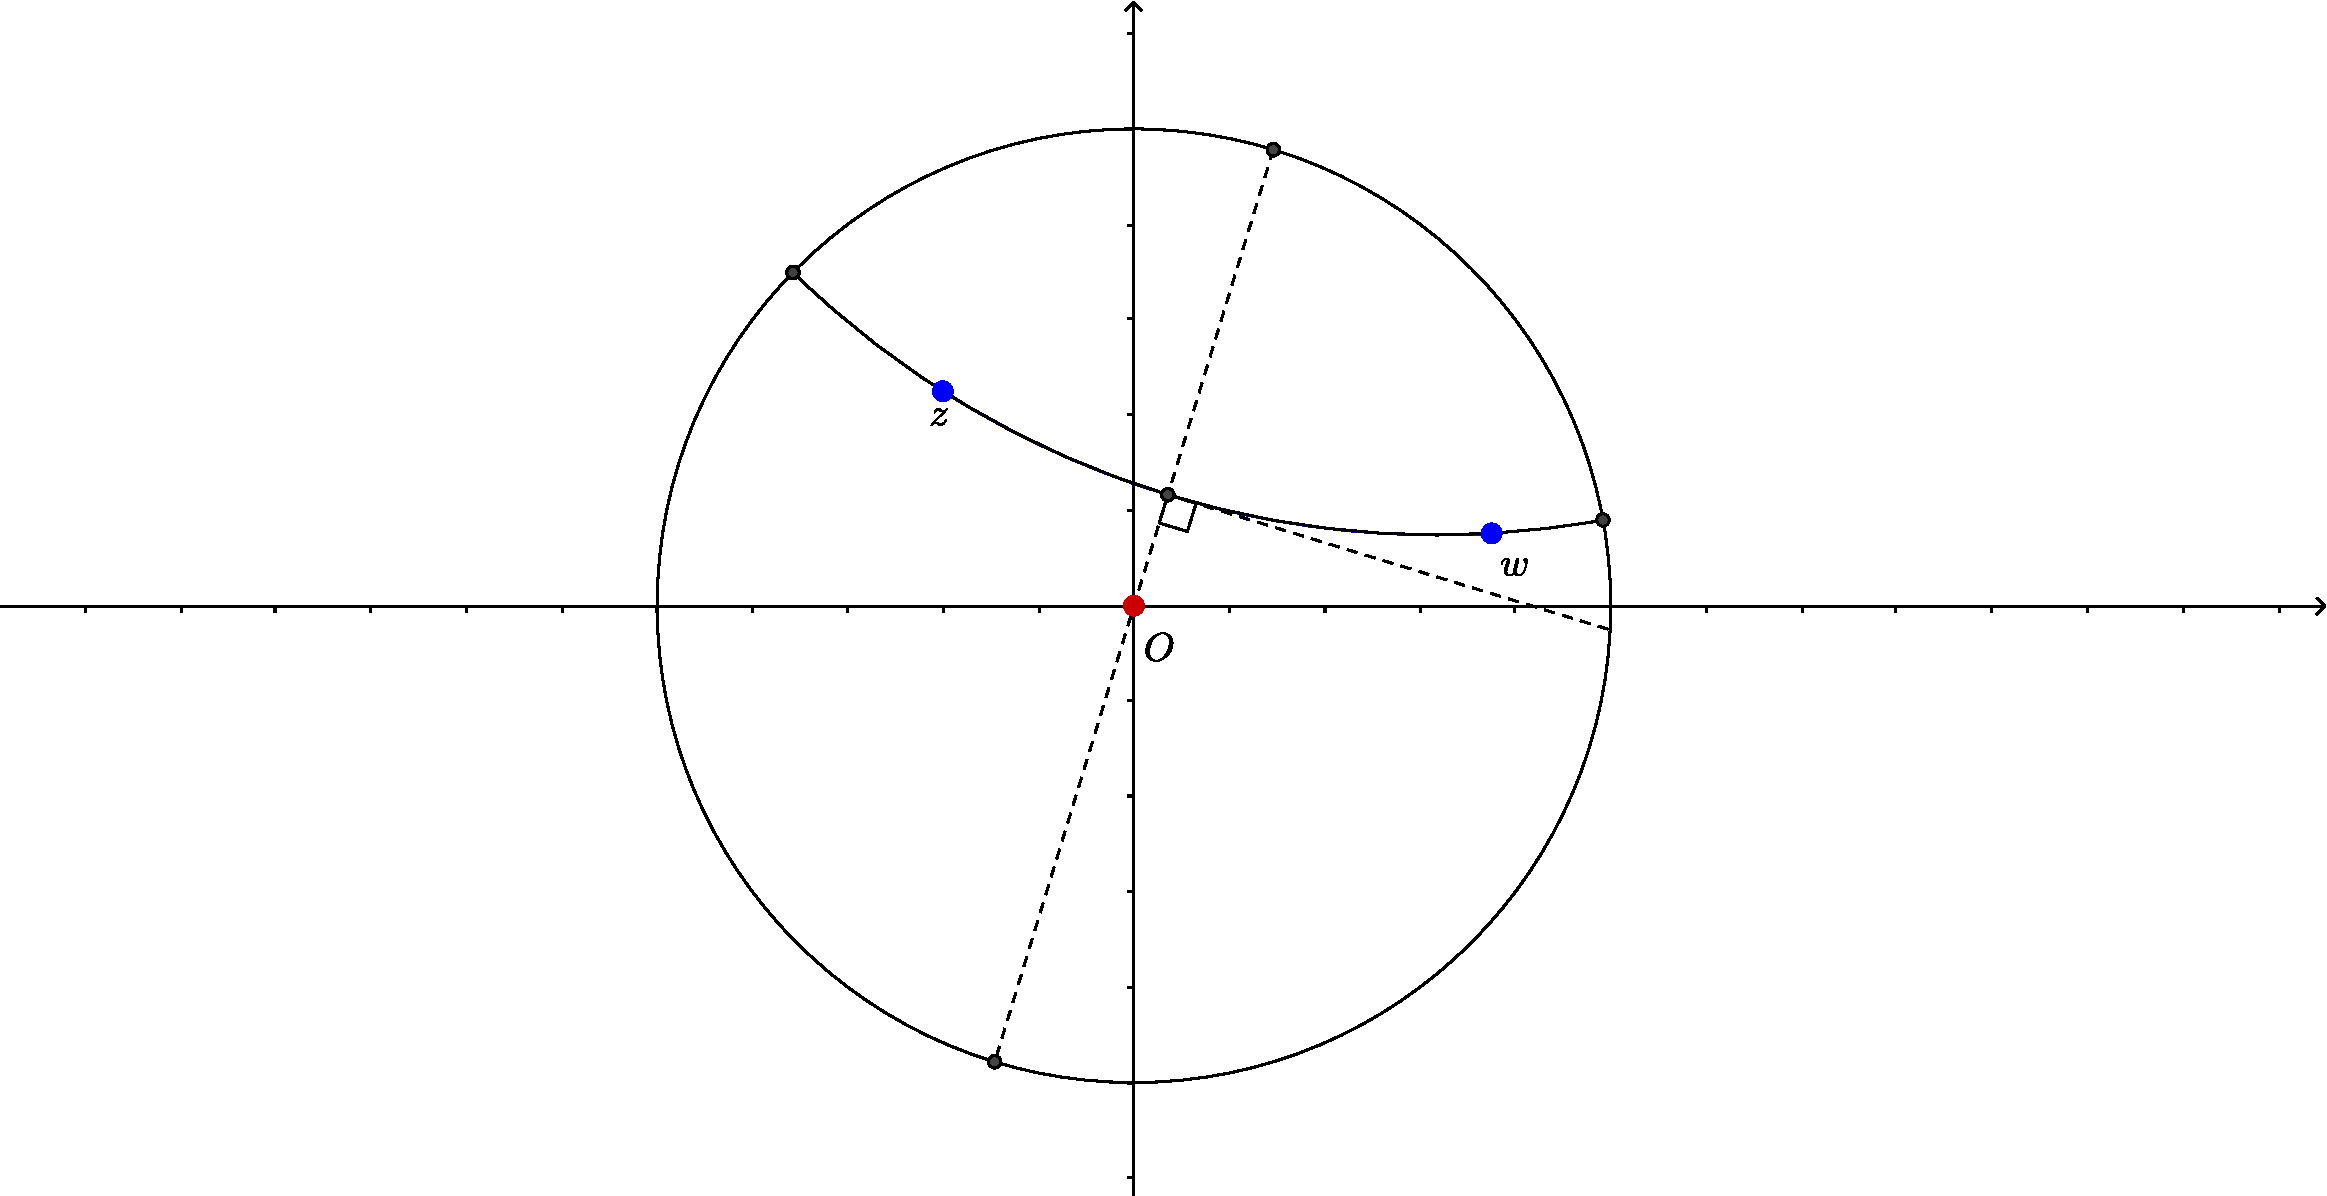
\includegraphics[width=\linewidth]{images/hyperbolic_disk_1.3.1.pdf}
        \caption{Trắc địa trong $\U$}
    \end{figure}
\end{thm}
\begin{proof}
    Nhắc lại ánh xạ phân tuyến tính $f(z)= \dfrac{iz+1}{z+i}$ là một vi phôi từ $\hh$ vào $\U$ nên nó biến biên $\partial(\hh)$ của $\hh$ thành biên $\partial(\U)$ và biến đường tròn cũng như đường thẳng trong $\C$ thành đường tròn và đường thẳng trong $\C$. Vì đường trắc địa trong $\hh$ là các nửa đường tròn hoặc đường thẳng vuông góc với trục thực (tức biên $\partial(\hh)$). Vì vậy nếu chỉ ra được $f$ là ánh xạ bảo giác (ta sẽ chứng minh ở các phần kế tiếp) thì ta sẽ chỉ ra được đường trắc địa trong $\U$ là các đoạn của các đường tròn Euclid trực giao với đường tròn đơn vị $\Sigma$ và các đường kính của nó.
\end{proof}
Tiếp theo ta đi xác định tất cả các phép biến đổi đẳng cự trên mặt phẳng hyperbolic.

Cho $PS^*L(2,\R) = S^*L(2,\R)/\{\pm I_2\}$ với $S^*L(2,\R) = \{A \in GL_2(\R)~|~\det(A) \in \{\pm 1\}\}$. Khi đó $\PSL(2,\R)$ là một nhóm con chỉ số 2 của $PS^*L(2,\R)$. Định lý sau xác định toàn bộ các phép biến đổi đẳng cự trên $\hh$.
\begin{thm}\label{thm 2.3.7}
    Nhóm các phép biến đổi đẳng cự $\Isom(\hh)$ được sinh bởi $\PSL(2,\R)$ và phép biến đổi $z\mapsto -\overline{z}$. Hơn nữa $\Isom(\hh) \cong PS^*L(2,\R)$.
\end{thm}
\begin{proof}
    Ta lần lượt có các khẳng định sau
    \begin{itemize}
        \item[i.] Với mỗi phép biến đổi đẳng cự $\varphi \in \Isom(\hh)$ thì $\varphi$ biến một đường trắc địa thành một đường trắc địa trong $\hh$.
        \item[ii.] Phép biến đổi $z\mapsto -\overline{z}$ cũng là một đẳng cự trong $\hh$.
    \end{itemize}
    Thật vậy, với mọi $z, w \in \hh$, khi đó với mọi $\xi \in [z,w]$ thì $\rho(z,w)= \rho(z,\xi)+\rho(\xi,w)$. Mà $\varphi$ là một phép biến đổi đẳng cự nên $\rho(\varphi(x),\varphi(y))=\rho(x,y)~\forall x,y\in \hh$. Dẫn đến $\rho(\varphi(z),\varphi(w)) = \rho(\varphi(z),\varphi(\xi)) + \rho(\varphi(\xi),\varphi(w))$, điều này tương đương với \[\varphi(\xi) \in [\varphi(z),\varphi(w)].\] Chứng tỏ $\varphi$ biến một đường trắc địa thành một đường trắc địa trong $\hh$. Do đó nếu kí hiệu $h-line(0,\infty)$ là trục ảo của $\hh$ thì $\varphi(h-line(0,\infty))$ là một đường trắc địa trong $\hh$. Mà tồn tại phép biến đổi $f \in \PSL(2,\R)$ biến đường trắc địa $\varphi(h-line(0,\infty))$ thành trục ảo $h-line(0,\infty)$, tức $(f\circ \varphi)(h-line(0,\infty)) = f(\varphi(h-line(0,\infty))) = h-line(0,\infty)$. 
    % Mặt khác vì $\PSL(2,\R) \subset \Isom(\hh)$ nên $f$ cũng là một đẳng cự trong $\hh$, dẫn đến $f\circ \varphi$ cũng vậy.
    % Từ đó suy ra với mọi đường trắc địa bất kỳ trong $\hh$, vì luôn tồn tại một phép biến đổi phân tuyến tính trong $\PSL(2,\R)$ biến nó thành $h-line(0,\infty)$, hợp của phép biến đổi đó với $f \circ \varphi$ cũng là một phép biến đổi đẳng cự trong $\hh$ và lại đưa về trường hợp đang xét ở trên.
    Bây giờ, với bất kì $z = x+iy \in \hh$, đặt $(f\circ \varphi)(z) = a+ib$. Khi đó với $ic \in h-line(0,\infty)$, ta có thể giả sử $f\circ \varphi$ giữ bất động trục ảo $h-line(0,\infty)$, tức $(f\circ \varphi)(ic) = ic \in h-line(0,\infty)$. Ta có
    \begin{align*}
        \rho(z,ic)
        = \rho((f\circ \varphi)(x+iy),(f\circ \varphi)(ic))
        = \rho(a+ib,ic)
    \end{align*}
    tương đương với 
    \begin{align*}
        \ln{\dfrac{|(x+iy)-\overline{ic}|+|(x+iy)-ic|}{|(x+iy)-\overline{ic}|-|(x+iy)-ic|}} &= \ln{\dfrac{|(a+ib)-\overline{ic}|+|(a+ib)-ic|}{|(a+ib)-\overline{ic}|-|(a+ib)-ic|}}\\
        % \dfrac{\dfrac{|(x+iy)-\overline{ic}|}{|(x+iy)-ic|}+1}{\dfrac{|(x+iy)-\overline{ic}|}{|(x+iy)-ic|}-1} &= \dfrac{\dfrac{|(a+ib)-\overline{ic}|}{|(a+ib)-ic|}+1}{\dfrac{|(a+ib)-\overline{ic}|}{|(a+ib)-ic|}-1}\\
        \dfrac{|(x+iy)-\overline{ic}|}{|(x+iy)-ic|} &= \dfrac{|(a+ib)-\overline{ic}|}{|(a+ib)-ic|}\\
        % ~(\text{vì hàm } h(t) = \dfrac{t+1}{t-1} \text{ đơn điệu})\\
        \dfrac{x^2+(y+c)^2}{x^2+(y-c)^2} &= \dfrac{a^2+(b+c)^2}{a^2+(b-c)^2}\\
        y(a^2 + b^2 + c^2) &= b(x^2+y^2+c^2)
    \end{align*}
    Đẳng thức trên đúng với mọi $c>0$ nên $b=y, a^2 = x^2$, tức $a+ib = x+iy$ hoặc $a+ib = -x+iy$. Nghĩa là $(f\circ \varphi)(z) = z$ hoặc $(f\circ \varphi)(z) = -\overline{z}$. Vì vậy hoặc $\varphi(z) = f^{-1}(z)$ thì $\varphi \in \PSL(2,\R)$, hoặc $\varphi(z) = f^{-1}(-\overline{z})$. Đặt $f(z) = \dfrac{\alpha z+\beta}{\gamma z+ \theta} \in \PSL(2,\R)$, khi đó $\varphi(z) = \dfrac{\alpha (-\overline{z})+\beta}{\gamma (-\overline{z})+ \theta} = \dfrac{-\alpha (\overline{z})+\beta}{-\gamma (\overline{z})+ \theta}$ với $(-\alpha) \theta - (-\gamma)\beta = -(\alpha \theta - \gamma \beta) = -1$, dẫn đến $\varphi \in PS^*L(2,\R)$. Rõ ràng $\Isom(\hh)$ được sinh bởi $\PSL(2,\R)$ và phép biến đổi $z\mapsto -\overline{z}$ và $\Isom(\hh) \cong PS^*L(2,\R)$.
\end{proof}
